 \documentclass[xcolor=dvipsnames,table]{beamer}

\usepackage{latexsym}
\usepackage[utf8]{inputenc}
\usepackage[brazil]{babel}
\usepackage{amssymb}
\usepackage{amsmath}
\usepackage{stmaryrd}
\usepackage{fancybox}
\usepackage{datetime}
\usepackage[T1]{fontenc}
\usepackage{graphicx}
\usepackage{graphics}
\usepackage{url}
\usepackage{algorithmic}
\usepackage{algorithm}
\usepackage{acronym}
\usepackage{array}

\usepackage{enumitem}

\newtheorem{definicao}{Definio}
\newcommand{\tab}{\hspace*{2em}}

\mode<presentation>
{
  \definecolor{colortexto}{RGB}{0,0,0}
 
  \setbeamertemplate{background canvas}[vertical shading][ bottom=white!10,top=white!10]
  \setbeamercolor{normal text}{fg=colortexto} 

  \usetheme{Warsaw}
}

\title{Agentes Inteligentes}  

\author{
  Esdras Lins Bispo Jr. \\ \url{bispojr@ufj.edu.br}
  } 
 \institute{
  Inteligência Artificial \\Bacharelado em Ciência da Computação}
\date{\textbf{24 de agosto de 2026} }

\logo{
\includegraphics[width=1.5cm]{images/ufjJataiLogo.png}}

\begin{document}

	\begin{frame}
		\titlepage
	\end{frame}

	\AtBeginSection{
		\begin{frame}{Sumário}%[allowframebreaks]{Sumário}
    		\tableofcontents[currentsection]
    		%\tableofcontents[currentsection, hideothersubsections]
		\end{frame}
	}

	\begin{frame}{Plano de Aula}
		\tableofcontents
		%\tableofcontents[hideallsubsections]
	\end{frame}
	
	\section{Instrução pelos Colegas}
	

    \begin{frame}{Pesquisa 002}
		\begin{block}{[P002]}
			Como foi a leitura do estudo prévio?
		\end{block}
		\begin{enumerate}[label=(\Alph*)]
			\item Boa leitura
			\item Leitura razoável
			\item Difícil de ler
			\item Não consegui ler
		\end{enumerate}
	\end{frame}

    \section{Agentes Inteligentes}
	\begin{frame}{Agentes Inteligentes}
		\begin{block}{Agente}
			Um {\color{blue} \bf agente} é tudo o que pode ser considerado capaz de perceber seu {\color{blue} \bf ambiente} por meio de {\color{blue} \bf sensores} e de agir sobre esse ambiente por intermédio de {\color{blue} \bf atuadores}.
		\end{block}	
	\end{frame}
	
	\begin{frame}{Agentes Inteligentes}
		\begin{center}
    		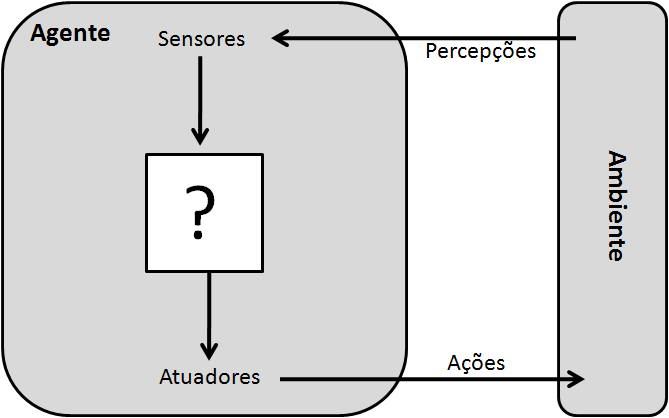
\includegraphics[width=.8\textwidth]{images/esquema.png}
  		\end{center}
	\end{frame}
	
	\begin{frame}{Agentes Inteligentes}
		\begin{block}{Agente}
			Um {\color{blue} \bf agente} é tudo o que pode ser considerado capaz de perceber seu {\color{blue} \bf ambiente} por meio de {\color{blue} \bf sensores} e de agir sobre esse ambiente por intermédio de {\color{blue} \bf atuadores}.
		\end{block}
		\begin{block}{Percepção}
			\begin{itemize}						
				\item O termo {\color{blue} \bf percepção} é uma referência às entradas perceptivas do agente em qualquer momento dado;
				\item Uma {\color{blue} \bf sequência de percepções} do agente é a história completa de tudo o que o agente já percebeu.
			\end{itemize}
		\end{block}
	\end{frame}
	
	\begin{frame}{Mundo do Aspirador de Pó}
		\begin{center}
    		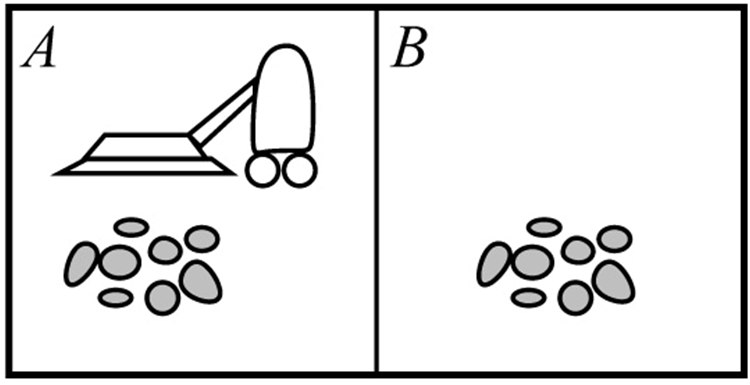
\includegraphics[width=.8\textwidth]{images/aspirador.png}
  		\end{center}
	\end{frame}
    
    \begin{frame}{Agentes Inteligentes}
		\begin{block}{Função de agente}
			É uma {\color{blue} \bf função} que descreve o comportamento do agente mapeando qualquer sequência de percepções específica para uma ação. 
		\end{block}	\pause
		\begin{block}{Programa de agente}
			\begin{itemize}						
				\item É uma {\color{blue} \bf implementação concreta} da descrição matemática abstrata da função de agente. Esta implementação {\color{blue} \bf depende da arquitetura} do agente.
			\end{itemize}
		\end{block}
	\end{frame}
	
	\begin{frame}{Mundo do Aspirador de Pó}
		\begin{center}
    		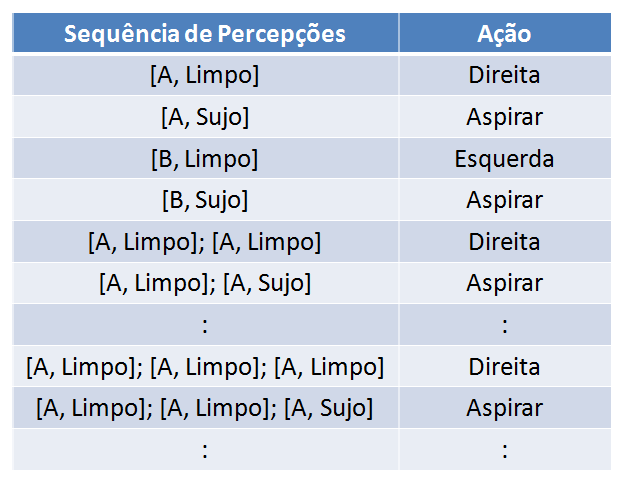
\includegraphics[width=.8\textwidth]{images/tabela.png}
  		\end{center}
	\end{frame}

	\begin{frame}{Questão 005} 
		\footnotesize
		\begin{block}{[Q005]} 
			Considere dois agentes que atuam no mesmo ambiente e recebem exatamente as mesmas percepções. O agente A implementa uma determinada função de agente por meio de uma tabela, enquanto o agente B implementa a mesma função por meio de um programa baseado em regras. Sobre essa situação, é correto afirmar que... 
		\end{block} 
		\begin{enumerate}[label=(\Alph*)] 
			\item A e B necessariamente produzem comportamentos diferentes, pois utilizam programas diferentes. 
			\item A e B podem produzir exatamente o mesmo comportamento, pois programas diferentes podem implementar a mesma função de agente. 
			\item A implementa uma função de agente, enquanto B implementa um programa de agente; portanto, apenas B possui comportamento definido. 
			\item A função de agente e o programa de agente são conceitos equivalentes, pois ambos recebem a percepção atual e retornam uma ação. 
		\end{enumerate} 
	\end{frame}


        \begin{frame}{Medida de Desempenho}
		\begin{block}{Medida de Desempenho}
			É um {\color{blue} \bf critério} para se medir o sucesso do agente.
		\end{block}	\pause
		\begin{block}{A racionalidade depende...}
			\begin{itemize}						
				\item Da {\color{blue} \bf medida de desempenho};
 				\item Do conhecimento anterior do agente sobre o {\color{blue} \bf ambiente};
 				\item Das {\color{blue} \bf ações} que o agente pode executar;
 				\item Da sequência de {\color{blue} \bf percepções} do agente até o momento.
			\end{itemize}
		\end{block}
	\end{frame}
	
	\begin{frame}{Logo a racionalidade é...}
		\begin{block}{}
			``Para cada {\color{blue} \bf sequência de percepções} possível, um agente racional deve selecionar uma {\color{blue} \bf ação} que venha maximizar sua {\color{blue} \bf medida de desempenho}, dada a evidência fornecida pela sequência de percepções e por qualquer {\color{blue} \bf conhecimento interno} do agente''.
		\end{block}
	\end{frame}

	\begin{frame}{Questão 006}
		\footnotesize

    \begin{block}{[Q006]}
        Um agente aspirador de pó foi projetado para:

        \begin{itemize}
            \item receber 1 ponto a cada instante em que um quadrado está limpo;
            \item pagar uma penalidade de 1 ponto sempre que se mover.
        \end{itemize}

        Depois que os dois quadrados já estão limpos, o agente continua
        alternando entre eles.

        Considerando essa nova medida de desempenho, qual avaliação
        é mais adequada?
    \end{block}

    \begin{enumerate}[label=(\Alph*)]

        \item O agente continua necessariamente racional, pois sua função
        de agente não mudou.

        \item O agente pode ter se tornado irracional, pois a racionalidade
        depende também da medida de desempenho adotada.

        \item O agente é irracional porque um agente racional nunca deve
        executar a mesma ação mais de uma vez.

        \item O agente continua racional, pois realizar mais ações sempre
        aumenta a experiência do agente.

    \end{enumerate}

\end{frame}
	
	\begin{frame}{Onisciência {\it versus} Racionalidade}
		\begin{block}{Onisciência}
			Um agente onisciente sabe o {\color{blue} \bf resultado real} de suas ações e pode agir de acordo em relação a ele.
		\end{block}	\pause
		\begin{block}{Racionalidade}
			Um agente racional sabe o {\color{blue} \bf resultado esperado} de suas ações e pode agir de acordo em relação a ele.
		\end{block}
	\end{frame}

	\begin{frame}{Questão 007}

		\small

    \begin{block}{[Q007]}
        Um agente precisa atravessar uma rua. Seus sensores ainda não
        permitem determinar se há veículos se aproximando.

        Um estudante afirma:

        \begin{quote}
        ``Como o agente não sabe o que acontecerá, qualquer ação que ele
        escolher será igualmente racional.''
        \end{quote}

        Qual resposta melhor explica por que essa afirmação está incorreta?
    \end{block}

    \begin{enumerate}[label=(\Alph*)]

        \item Um agente racional deve sempre escolher a ação que produz
        o melhor resultado real.

        \item Um agente racional não pode agir em ambientes parcialmente
        observáveis.

        \item O agente deve considerar que ações (como obter mais informação) podem aumentar seu desempenho esperado antes da decisão.

        \item Se o resultado não puder ser conhecido com certeza, a única
        escolha racional é não fazer nada.

    \end{enumerate}

\end{frame}

	
	
	\begin{frame}
		\titlepage
	\end{frame}
	
\end{document}